\documentclass[10pt,a4paper]{article}
\usepackage[margin=0.67in]{geometry}
\usepackage[T1]{fontenc}
\usepackage{lmodern}
\usepackage{microtype}
\usepackage{amsmath,booktabs,array,tikz,xcolor}
\usepackage[hidelinks]{hyperref}
\usepackage{enumitem}
\setlength{\parindent}{0pt}
\setlength{\parskip}{3pt}
\makeatletter
\renewcommand\section{\@startsection{section}{1}{0pt}{1.5ex plus .3ex minus .1ex}{.6ex plus .1ex}{\normalfont\normalsize\bfseries}}
\makeatother
\setlength{\tabcolsep}{6pt}
\definecolor{blue}{HTML}{0072B2}
\definecolor{orange}{HTML}{D55E00}
\definecolor{green}{HTML}{009E73}
\definecolor{gray}{HTML}{707070}
\definecolor{ink}{HTML}{20262E}
\hypersetup{pdftitle={JSON Serialization Sensitivity of Released SuperBPE Tokenizers: Synthetic and Public-Artifact Evidence},pdfauthor={Zhijing Wu},pdfsubject={Independent Technical Note draft; no peer-review or affiliation claim}}
\begin{document}
\color{ink}
\begin{center}
{\fontsize{16}{19}\selectfont\bfseries JSON Serialization Sensitivity of Released\\
SuperBPE Tokenizers: Synthetic and Public-Artifact Evidence\par}
\vspace{4pt}
{\normalsize Zhijing Wu\par}
{\small Independent Technical Note draft \textbullet\ 14 October 2026\par}
\end{center}
\vspace{-5pt}

\textbf{Abstract.}
We measure how semantics-preserving JSON whitespace changes the relative token
savings of fixed, released 200k-vocabulary tokenizers. A frozen synthetic pilot
finds an indent-2 minus compact difference of \(6.72\) percentage points (pp),
with a 95\% cluster-bootstrap interval \([6.48,7.00]\).
A separate public-artifact evaluation gives an equal-source difference of
\(15.34\) pp, conditional interval \([14.37,16.30]\); 184 of its 208 objects
are protocol schemas and only 24 are agent arguments/states from two tasks.
The no-whitespace baseline beats t180k on 201/208 indented objects.
Byte partitions and vocabulary coverage support a structural-formatting
explanation, including an already documented colon-space restriction.
These are count measurements, not language-model or deployment-performance results.

\section*{\normalsize 1\quad Question and original-paper context}
Liu et al.\ introduced SuperBPE's curriculum from subword to
cross-whitespace superword learning, and evaluated trained language models [1].
Their digit, colon-space and boundary controls, and subsequent regex discussions
[1,2,3], motivate a narrower question here:
\emph{does serialization whitespace change the compression advantage of a
fixed released tokenizer on unchanged JSON objects?}
We independently evaluate the released assets; we do not reproduce the paper's
training corpus, LM results, or isolate the curriculum as a single causal variable.

\section*{\normalsize 2\quad Two separate frozen evaluations}
Both evaluations use the official BPE 200k and SuperBPE t180k assets at commit
\texttt{bbd09768fc28}, with t80k and no-whitespace 200k as sensitivities.
Python 3.13.5 and upstream \texttt{tokenizers==0.20.3} load the unchanged
normalizers, pretokenizers, vocabularies and merge ranks. The audited in-memory
adapter removes added tokens and supplies a ByteLevel decoder; dropout,
padding, truncation and special-token insertion are disabled.
All 5,248 original tokenizer/record/format observations pass exact decode,
deterministic-repeat, adapter-ID-parity and byte-reconstruction checks.
Full custom-fork parity remains unverified.

\emph{Synthetic pilot.} Seed 1729 generates 120 semantic families in four
balanced categories: tool arguments, schemas, execution records and inter-agent
messages. Twenty families are development-only; 100 held-out families
(25/category) determine the frozen endpoint. Each family has compact, spaced,
indent-2 and tab-indent forms, with sorted keys, UTF-8 preserved and no trailing
newline. Every form parses to the same object. Ten declared schema lineages per
category account for related content siblings.

\emph{Public artifacts.} A separately frozen set contains 91 MCP definition
objects [4], 93 A2A definition objects [5], and 18 tool-argument plus six
execution-state objects from published SWE-agent examples [6].
Exact canonical deduplication removes 37 repeated objects; two code-bearing
arguments are excluded for unverified underlying-source reuse rights before
counts. Existing values and array order are preserved. The same four formats
are used. The schema fragments retain reference context in their source
documents; they are not independent executions. All runtime replays belong to
only two benchmark tasks. Nothing is pooled with the synthetic endpoint.

\[
G(i,f)=1-\frac{N_{\mathrm{t180k}}(i,f)}{N_{\mathrm{BPE}}(i,f)},\qquad
D(i)=G(i,\mathrm{indent2})-G(i,\mathrm{compact}).
\]
The synthetic estimate averages categories equally; the external estimate
averages the three sources equally, with equal-record means within source.
Both use 10,000 paired whole-lineage bootstrap resamples (seed 6198),
with percentile 95\% intervals. External groups comprise ten MCP groups,
eight A2A groups and two SWE-agent tasks. External intervals condition on
these selected groups/sources and are not deployment-population intervals.

\begin{center}
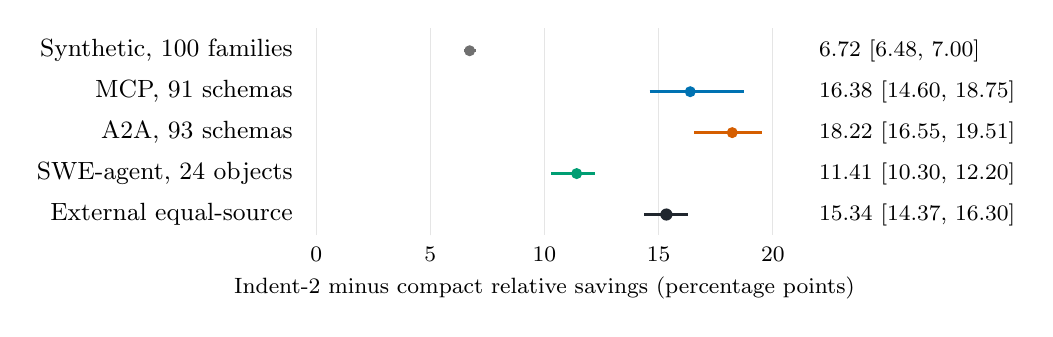
\begin{tikzpicture}[x=0.29cm,y=0.52cm,font=\small]
\draw[gray!30] (0,-0.5)--(0,4.55);
\draw[gray,densely dotted] (5,-0.5)--(5,4.55);
\foreach \x in {0,5,10,15,20} {
  \draw[gray!18] (\x,-0.5)--(\x,4.55);
  \node[below,font=\footnotesize] at (\x,-0.55) {\x};
}
\foreach \y/\name in {4/{Synthetic, 100 families},3/{MCP, 91 schemas},2/{A2A, 93 schemas},1/{SWE-agent, 24 objects},0/{External equal-source}} {
  \node[anchor=east] at (-0.6,\y) {\name};
}
\draw[gray,line width=1.2pt] (6.475239,4)--(7.000865,4);
\fill[gray] (6.721989,4) circle (2pt);
\draw[blue,line width=1.2pt] (14.599629,3)--(18.753538,3);
\fill[blue] (16.382660,3) circle (2pt);
\draw[orange,line width=1.2pt] (16.547061,2)--(19.509306,2);
\fill[orange] (18.222307,2) circle (2pt);
\draw[green,line width=1.2pt] (10.297422,1)--(12.201641,1);
\fill[green] (11.408216,1) circle (2pt);
\draw[ink,line width=1.2pt] (14.373616,0)--(16.296536,0);
\fill[ink] (15.337728,0) circle (2.2pt);
\foreach \y/\value in {4/{6.72 [6.48, 7.00]},3/{16.38 [14.60, 18.75]},2/{18.22 [16.55, 19.51]},1/{11.41 [10.30, 12.20]},0/{15.34 [14.37, 16.30]}} {
  \node[anchor=west,font=\footnotesize] at (21.6,\y) {\value};
}
\node[font=\footnotesize] at (10,-1.8) {Indent-2 minus compact relative savings (percentage points)};
\end{tikzpicture}
\end{center}
\vspace{-6pt}
{\footnotesize \textbf{Figure 1.} Separate finite-set effects and their respective
cluster-bootstrap intervals. The dotted 5 pp line is the synthetic pilot's
frozen practical reference, not a new external decision threshold.
The SWE-agent interval resamples only two task clusters.}

\newpage
\section*{\normalsize 3\quad Absolute costs, ranking reversal and consistency}
The synthetic interval exceeds its frozen \(+5\) pp margin, supporting
practical sensitivity \emph{within that fixture design}.
Externally, 207/208 object effects and all 20 group means are positive;
empty submit arguments give zero. The runtime-only estimate is \(11.41\) pp.
Pooled equal-record and corpus contrasts are \(16.63\) and \(15.71\) pp,
distinct from the \(15.34\) pp equal-source summary.

\begin{center}
\small
\begin{tabular}{llrrr}
\toprule
Set & Format & BPE tokens & t180k tokens & No-whitespace tokens\\
\midrule
Synthetic, 100 & Compact & 26,505 & 23,657 & 23,304\\
 & Indent-2 & 31,680 & 26,247 & 24,083\\
External, 208 & Compact & 24,624 & 22,462 & 25,625\\
 & Indent-2 & 41,378 & 31,246 & 26,757\\
\bottomrule
\end{tabular}
\end{center}
\vspace{-4pt}
{\footnotesize \textbf{Table 1.} Exact totals; a larger relative advantage can
coexist with more tokens per unchanged semantic object. All four formats and
t80k counts are available in the accompanying saved results.}

Indent-2 increases external bytes from 114,221 to 145,621 (\(+27.49\%\))
and t180k tokens by 8,784 (\(+39.11\%\)).
No-whitespace is worse than t180k in the compact external corpus, but better
on 201/208 indent-2 objects (five ties, two t180k wins), saving 4,489 tokens
relative to t180k in total. The synthetic counterpart is 99/100 objects.
t180k also regresses against ordinary BPE on one compact and 16 spaced
external objects; none regress under indent-2 or tab-indent.
There is no universal ranking or justification for adding whitespace to
minimize t180k's absolute token count.

\section*{\normalsize 4\quad Observational mechanism evidence}
Tokens qualify as spanning only if an original BPE pretoken boundary falls
inside their reconstructed byte span; a leading space alone is insufficient.
t180k's external crossing fraction rises from \(8.40\%\) to \(35.04\%\);
no-whitespace rises from \(26.23\%\) to \(62.59\%\).
More crossings coexist with worse compact counts, so frequency alone does
not explain efficiency.

The two assets share inference pretokenizers and non-vocabulary settings,
but only 32,883 of 200,000 byte-token strings.
A post-count static audit finds 893 no-whitespace colon-space token types
and zero in t180k, t80k or BPE, consistent with the documented intentional
restriction [1, Appendix A.1.4; 2,3].
The recorded substring
\verb|"type": "| costs four t180k tokens versus one no-whitespace token;
the complete token is absent from t180k's vocabulary.

Aligning the two emitted partitions at common byte boundaries conserves the
whole-record gap for all 832 external record/format pairs.
In indent-2, structural-only regions contribute \(+1{,}653\) tokens and
mixed structural-space regions \(+2{,}445\) to the no-whitespace advantage.
Regions containing structural colon-space carry 3,335 of the 4,489 net
gap. Such regions also contain other bytes and merge opportunities:
the accounting is observational, not a causal percentage attribution.
Different vocabularies and historical training constraints prevent a
curriculum-only causal conclusion.

\section*{\normalsize 5\quad Limitations and reproducibility}
The synthetic suite reuses authored phrases and shapes. The external set
is a convenience sample dominated by schemas; two curated runtime tasks
do not establish production-scale generalization. Shared standards cross
the declared groups. Source weighting and field lengths affect magnitude:
external leave-one-source means span \(13.90\) to \(17.30\) pp, while
longer string-value strata generally have smaller effects.
No reasoning, accuracy, inference-latency or commercial-billing improvement
is measured. No priority, UW affiliation or peer-review claim is made.

The \href{https://github.com/ZhijingWu/superbpe-serialization-evaluation}{accompanying repository}'s \texttt{README.md} and
\texttt{docs/reproducibility.md} provide standard-library replay of saved
counts and safe lineage metadata; both original analyses reproduce exactly.
Pinned upstream inputs are linked, with raw-LF/Windows-CRLF hashes distinguished.
Synthetic inputs and their generator remain private by owner decision:
statistical replay is available; full synthetic re-encoding requires private access.
Original included project materials use MIT; upstream rights remain separate.
Neither broader-task validation nor a boundary intervention was run in this stage.

{\footnotesize AI assistance was used in implementation and drafting.
All numerical claims were verified against preserved evidence.
This document is an independent Technical Note draft, not a peer-reviewed publication.}

\vspace{-3pt}
\begin{thebibliography}{6}
\footnotesize\setlength{\itemsep}{0pt}\setlength{\parskip}{0pt}
\bibitem{paper} A. Liu, J. Hayase, V. Hofmann, S. Oh, N. A. Smith and Y. Choi.
\emph{SuperBPE: Space Travel for Language Models}.
\href{https://arxiv.org/abs/2503.13423v3}{arXiv:2503.13423v3}, COLM 2025 camera-ready.
\bibitem{faq} SuperBPE authors. \href{https://superbpe.github.io/faq.html}{Official FAQ}.
\bibitem{issue} SuperBPE authors.
\href{https://github.com/PythonNut/superbpe/issues/9}{Stage-2 punctuation/newline discussion, issue 9}.
\bibitem{mcp} MCP project.
\href{https://github.com/modelcontextprotocol/modelcontextprotocol/blob/3778656b2e0ba6725035e816fe3085374cbaa736/schema/2025-06-18/schema.json}{JSON Schema 2025-06-18, pinned source snapshot}.
\bibitem{a2a} A2A project.
\href{https://github.com/a2aproject/A2A/blob/8d57eba286de756176892518a8fc39b0ac2ccefb/specification/json/a2a.json}{Protocol JSON Schema v0.3.0}.
\bibitem{swe} SWE-agent project.
\href{https://github.com/SWE-agent/SWE-agent/tree/3ea751c087f32b16e039a2233dd6eefecef325d5}{Published demonstrations and test trajectories, pinned snapshot}.
\end{thebibliography}
\end{document}
